\documentclass[aspectratio=169]{beamer}
\setbeamertemplate{navigation symbols}{}
\usepackage{color, amsmath, comment, subfigure}
\usepackage{url}
\usepackage{tikz}

\usepackage{hyperref}
\hypersetup{
    colorlinks=true,
    linkcolor=blue,
    filecolor=magenta,      
    urlcolor=cyan,
}

\newcommand\red[1]{{\color{red}#1}}
\newcommand\bred[1]{{\color{red}\textbf{#1}}}
\newcommand\blue[1]{{\color{blue}#1}}
\newcommand\bblue[1]{{\color{blue}\textbf{#1}}}
\newcommand\green[1]{{\color{olive}#1}}
\newcommand\bgreen[1]{{\color{olive}\textbf{#1}}}
\newcommand\black[1]{{\color{black}#1}}
\newcommand\white[1]{{\color{white}#1}}
\newcommand\E{\text{E}}
\newcommand\V{\text{V}}
\renewcommand\P{\text{P}}


%%%%%%%%%%%%%%%%%%%%%%%%%%
\title[]{Class slides for Tuesday, November 10:\\Predictability of life trajectories}
\author[]{Matthew J. Salganik}
\institute[]{}
\date[]{COS 597E/SOC 555 Limits to prediction\\Fall 2020, Princeton University}

\begin{document}
%%%%%%%%%%%%%%%%%%%%%%%%%%%
\frame{\titlepage}
%%%%%%%%%%%%%%%%%%%%%%%%%%%
\begin{frame}

\begin{center}
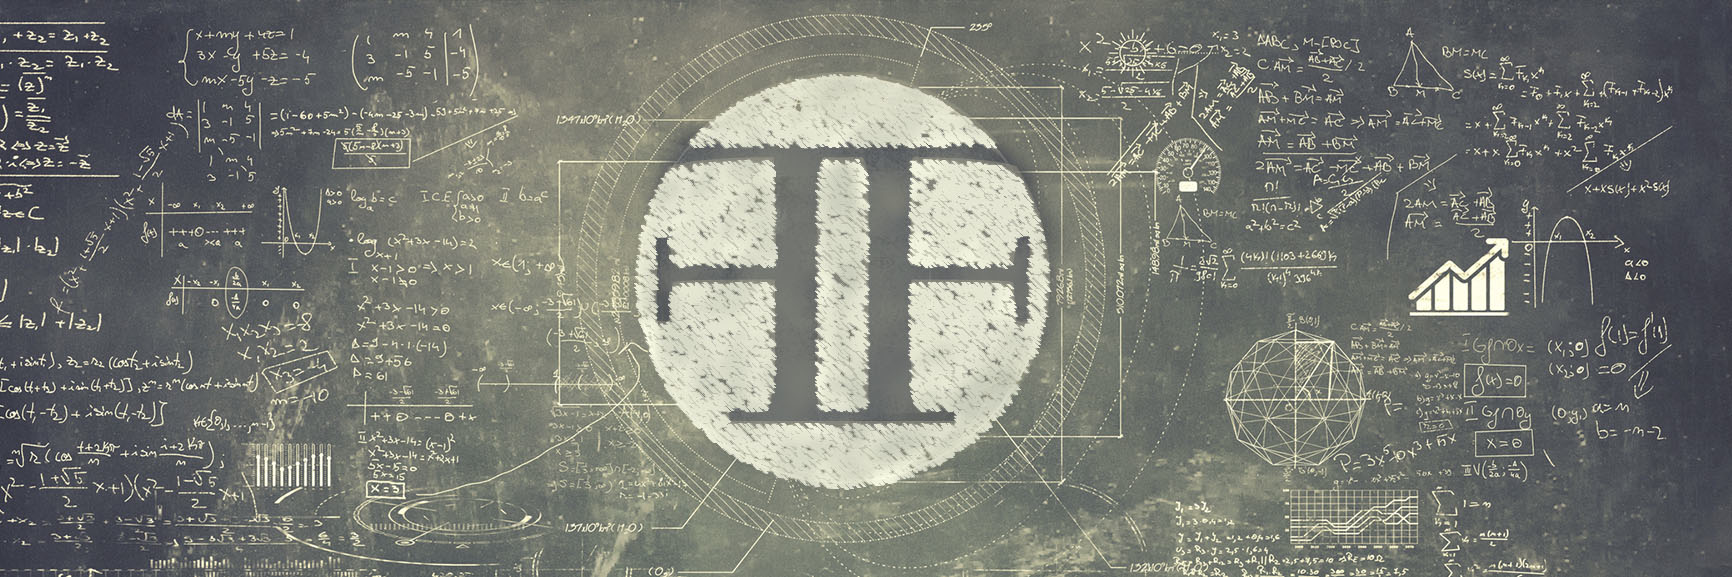
\includegraphics[width=\textwidth]{figures/ffc_masthead}
\Large{Fragile Families Challenge}
\end{center}

\end{frame}
%%%%%%%%%%%%%%%%%%%%%%%%%%%
\begin{frame}

\begin{center}
\Huge{
$ \hat{y} \quad \& \quad \hat{\beta}$
}
\end{center}

\vfill
\tiny{Mullainathan and Spiess (2017)}
\end{frame}
%%%%%%%%%%%%%%%%%%%%%%%%%%
\begin{frame}

\begin{center}

\includegraphics[width=\textwidth]{figures/ff_logo}
\end{center}

\begin{itemize}
\item Birth cohort panel study
\item $\approx$ 5,000 children born in 20 U.S. cities with an over-sample of non-marital births
\item Followed from birth through age 15
\item Already used in hundreds of papers and dozens of dissertations
\end{itemize}

\end{frame}
%%%%%%%%%%%%%%%%%%%%%%%%%%%
\begin{frame}

\begin{center}
\only<1>{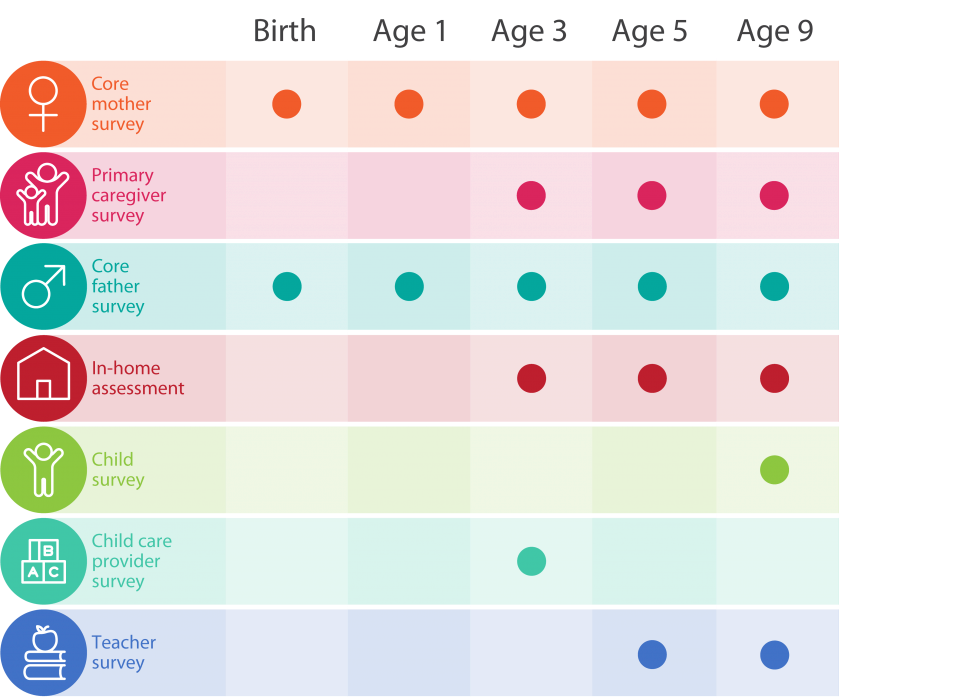
\includegraphics[width=0.8\textwidth]{figures/ff_design_public_b9}}
\only<2>{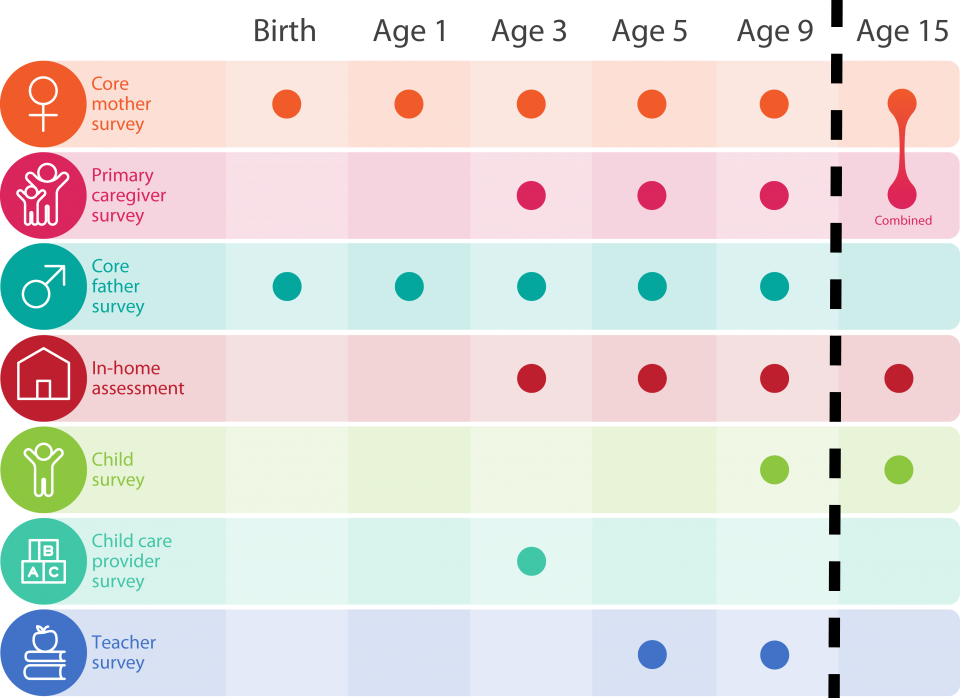
\includegraphics[width=0.8\textwidth]{figures/ff_design_public2}}
\end{center}

\end{frame}
%%%%%%%%%%%%%%%%%%%%%%%%%
\begin{frame}

\begin{center}
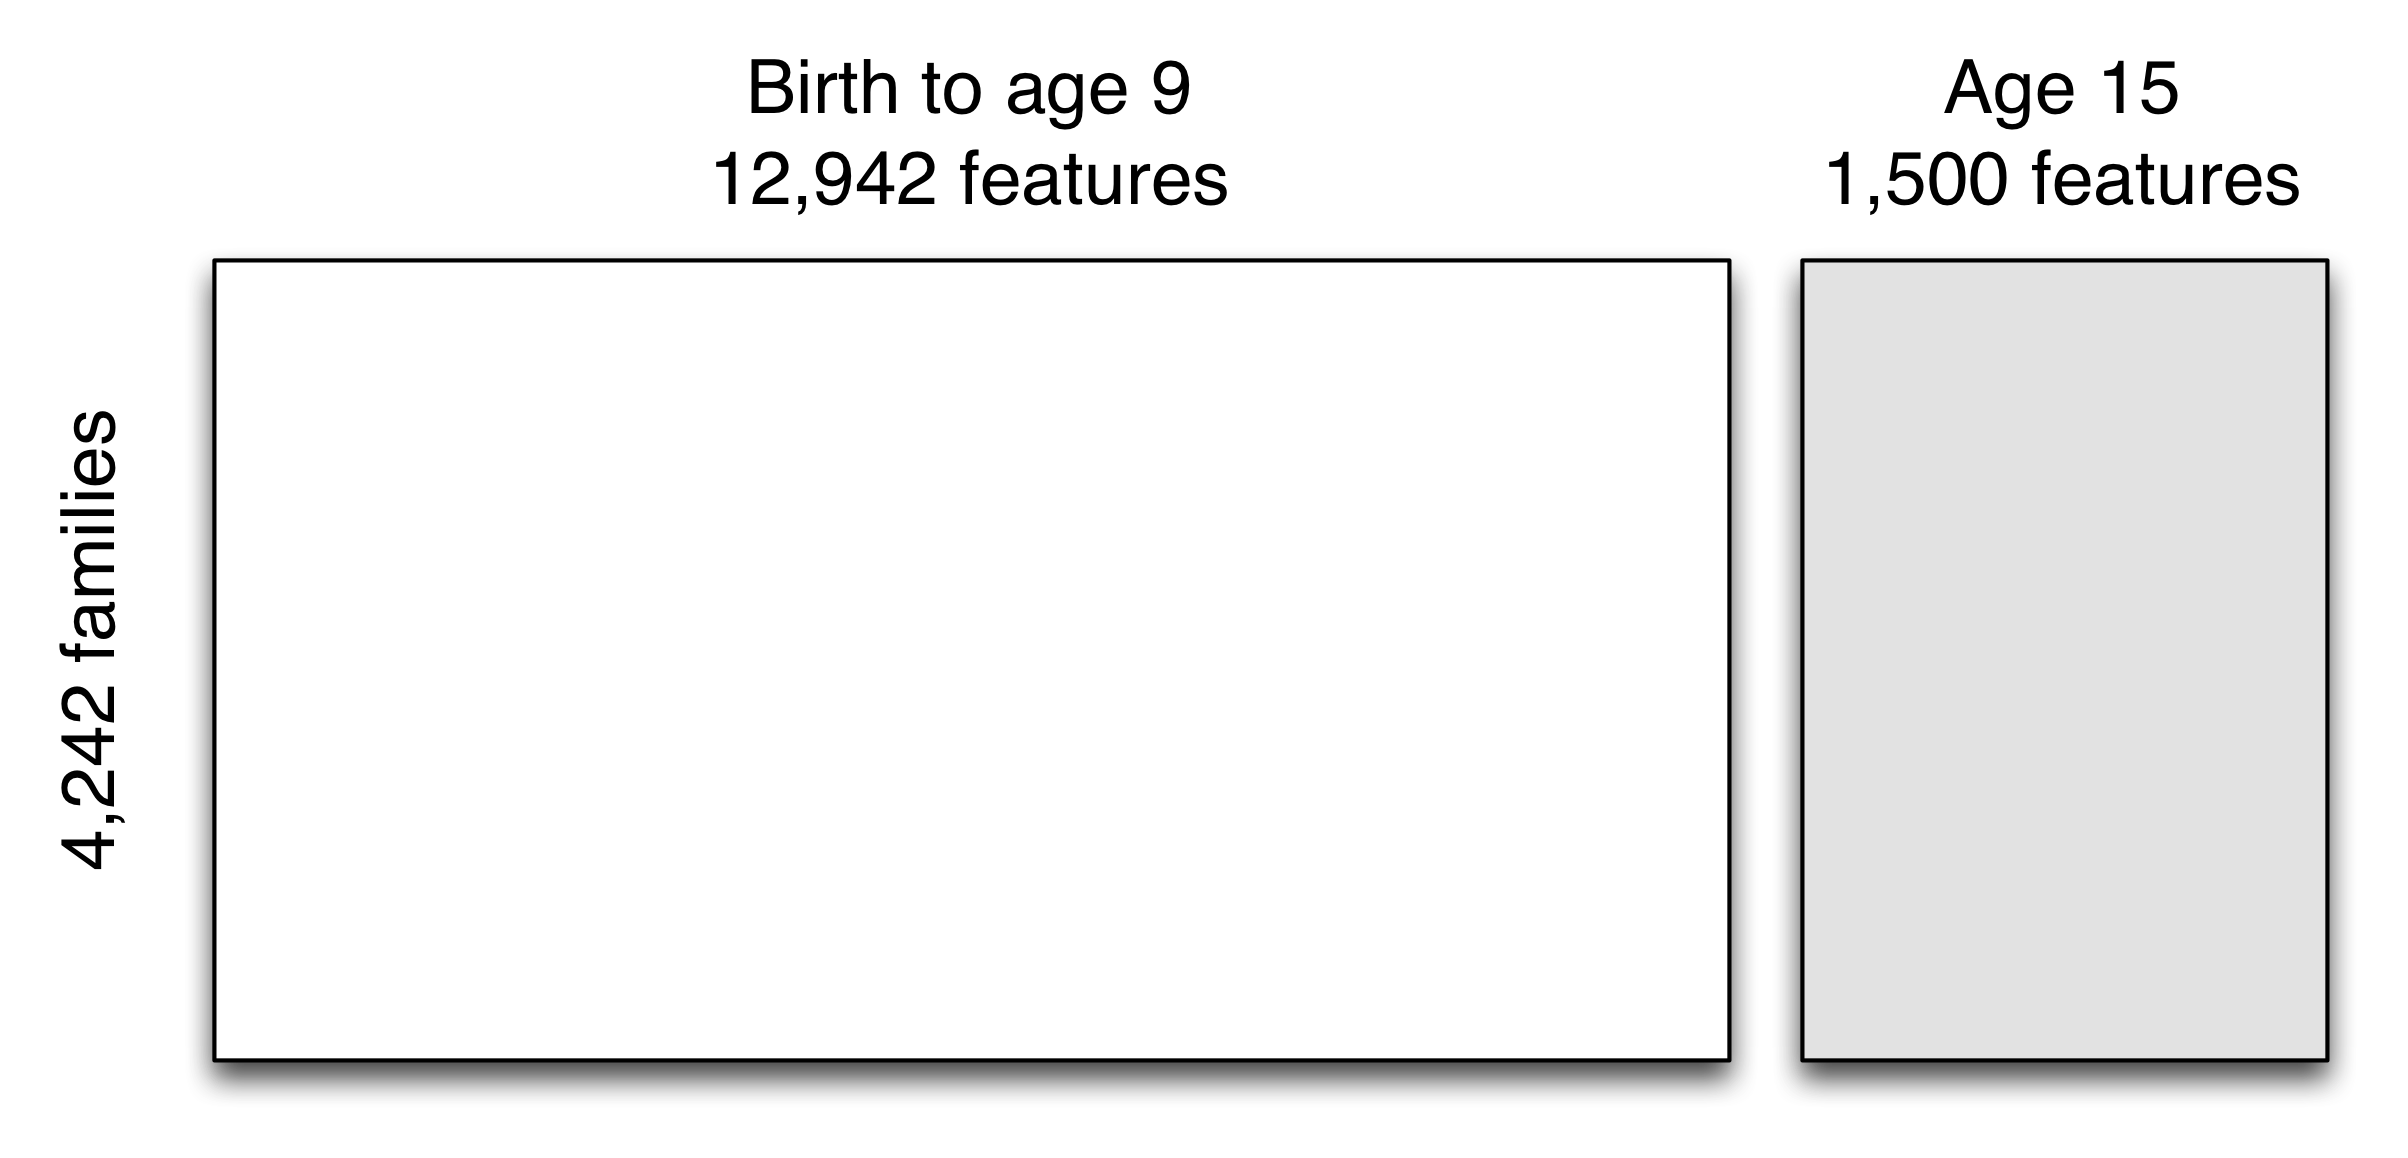
\includegraphics[width=\textwidth]{figures/ff_design_matrix_ml}
\end{center}

\end{frame}
%%%%%%%%%%%%%%%%%%%%%%%%%
\begin{frame}

\begin{center}
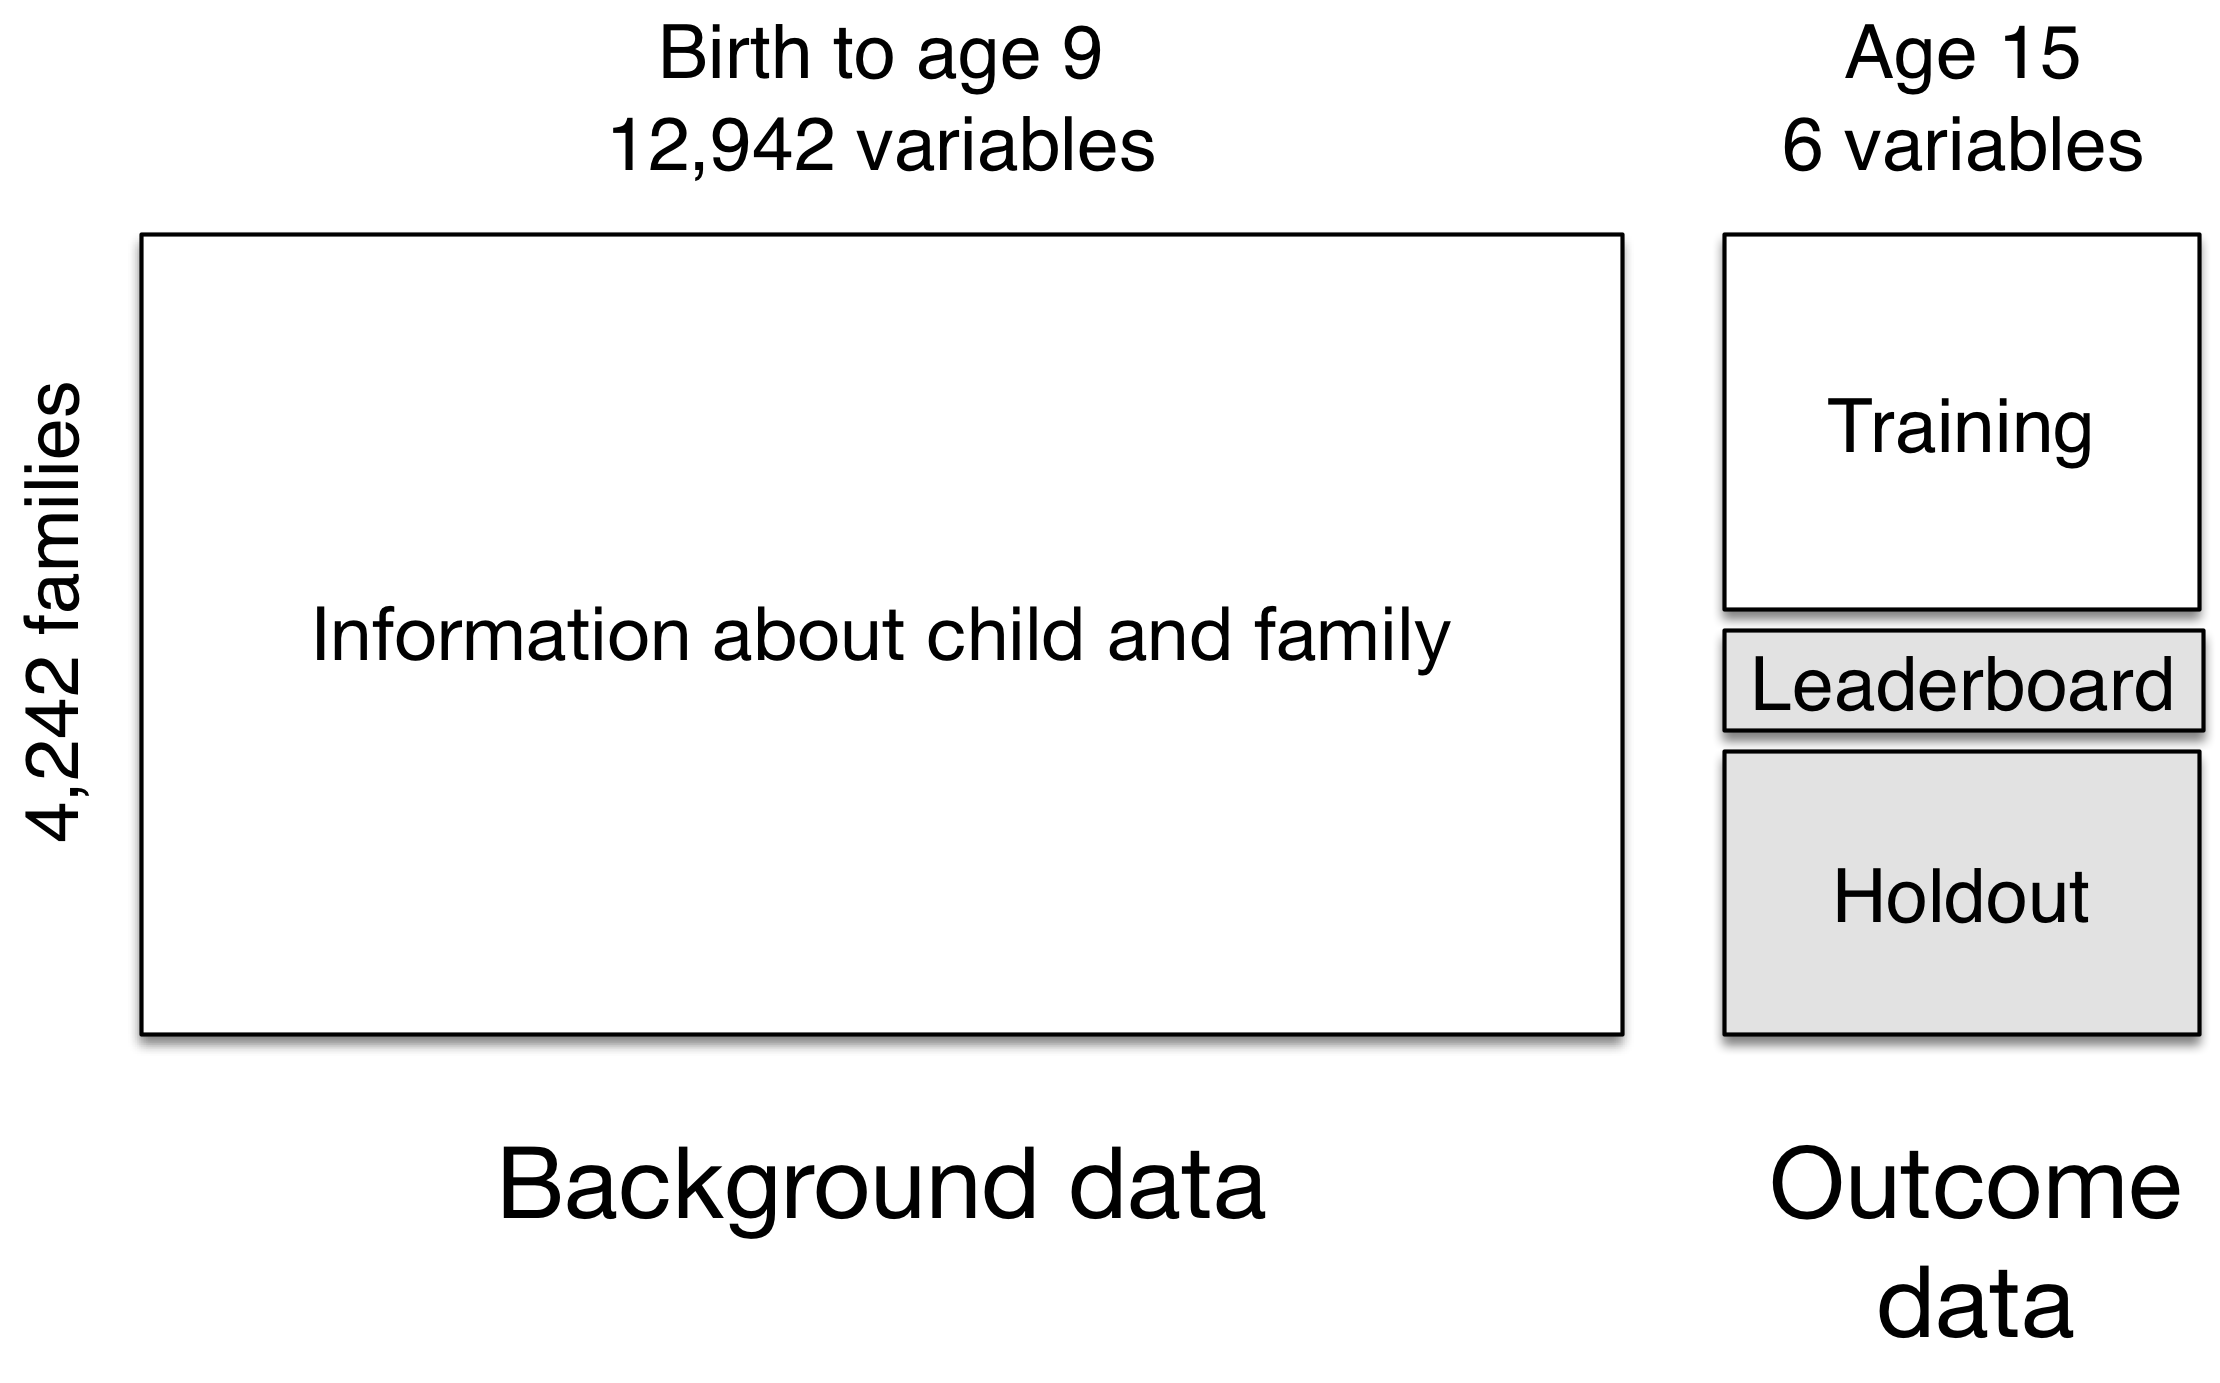
\includegraphics[width=0.8\textwidth]{figures/ffc_design_matrix_ml}
\end{center}

\vfill
This is not inferring the present or forecasting. What is it?

\end{frame}
%%%%%%%%%%%%%%%%%%%%%%%%%
\begin{frame}

Outcomes
\begin{itemize}
\item Child: GPA (continuous), Grit (continuous)
\item Household:  Eviction (binary), Material hardship (continuous)
\item Primary care giver: Job training (binary), Job loss (binary)
\end{itemize}

\end{frame}
%%%%%%%%%%%%%%%%%%%%%%%%%
\begin{frame}

457 researchers applied to participate. Many worked in interdisciplinary teams. Goal: Make a prediction that minimizes mean square error on the hold-out set
\begin{equation*}
MSE_{\text{holdout}} = \frac{\sum_{i \in \text{holdout}} (\hat{y}_i - y_i)^2}{n_{holdout}}
\end{equation*}

\vfill
More on privacy and ethics audit: Lundberg et al.\ (2019)
\end{frame}
%%%%%%%%%%%%%%%%%%%%%%%%%
\begin{frame}

Using a large, high-quality social science dataset collected since birth and modern machine learning methods, how accurately can we predict outcomes from children, parents, and families?

\begin{equation*}
R^2_{holdout} = 1 - \frac{\sum_{i \in \text{holdout}} (\hat{y}_i - y_i)^2}{\sum_{i \in \text{holdout}} (\bar{y}_{train} - y_i)^2}
\end{equation*}

\pause 
\vfill

Before I show the results, let's vote . . . . (Also notice the switch from absolute to relative metric)

\end{frame}
%%%%%%%%%%%%%%%%%%%%%%%%%
\begin{frame}

\begin{center}
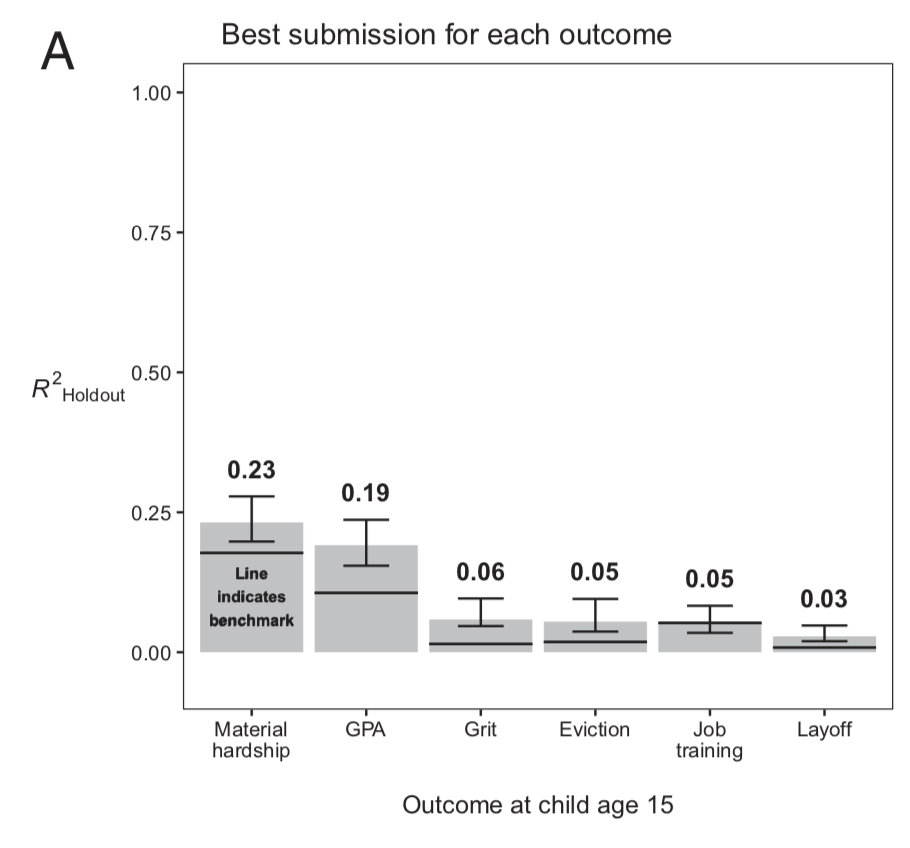
\includegraphics[width=0.5\textwidth]{figures/salganik_measuring_2020_fig3a}
\end{center}

\pause
\vfill
What is the right y-scale here?

\end{frame}
%%%%%%%%%%%%%%%%%%%%%%%%%%
\begin{frame}

\begin{center}
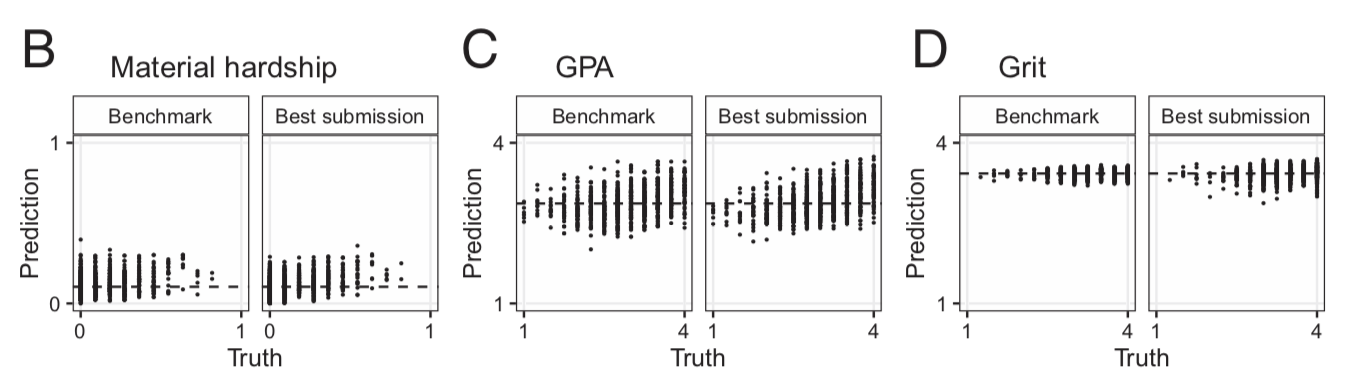
\includegraphics[width=\textwidth]{figures/salganik_measuring_2020_fig3b-d}
\end{center}

\begin{itemize}
\item Best submission is like the mean of the training data with a bit of signal, not like the truth with a bit of noise
\item Best submission is qualitatively similar to the benchmark model 
\end{itemize}

\end{frame}
%%%%%%%%%%%%%%%%%%%%%%%%%%
\begin{frame}

\begin{center}
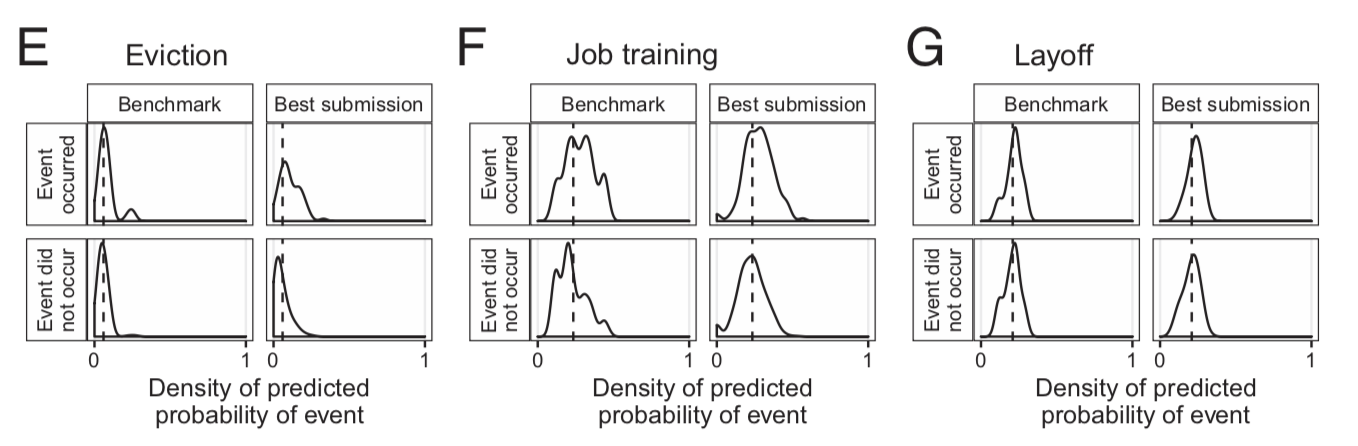
\includegraphics[width=\textwidth]{figures/salganik_measuring_2020_fig3e-g}
\end{center}

\begin{itemize}
\item Best submission is like the mean of the training data with a bit of signal, not like the truth with a bit of noise
\item Best submission is qualitatively similar to the benchmark model 
\end{itemize}

\end{frame}
%%%%%%%%%%%%%%%%%%%%%%%%%%
\begin{frame}

We can learn a lot by looking at all the valid submissions, not just the best

\end{frame}
%%%%%%%%%%%%%%%%%%%%%%%%%
\begin{frame}

\begin{center}
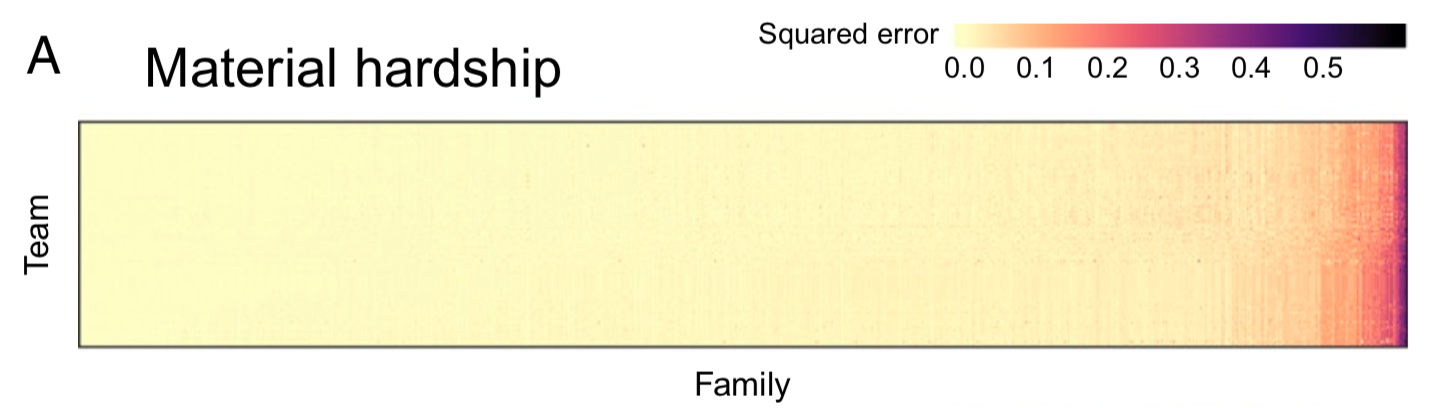
\includegraphics[width=\textwidth]{figures/salganik_measuring_2020_fig4a}
\end{center}

\end{frame}
%%%%%%%%%%%%%%%%%%%%%%%%%%
\begin{frame}

\begin{center}
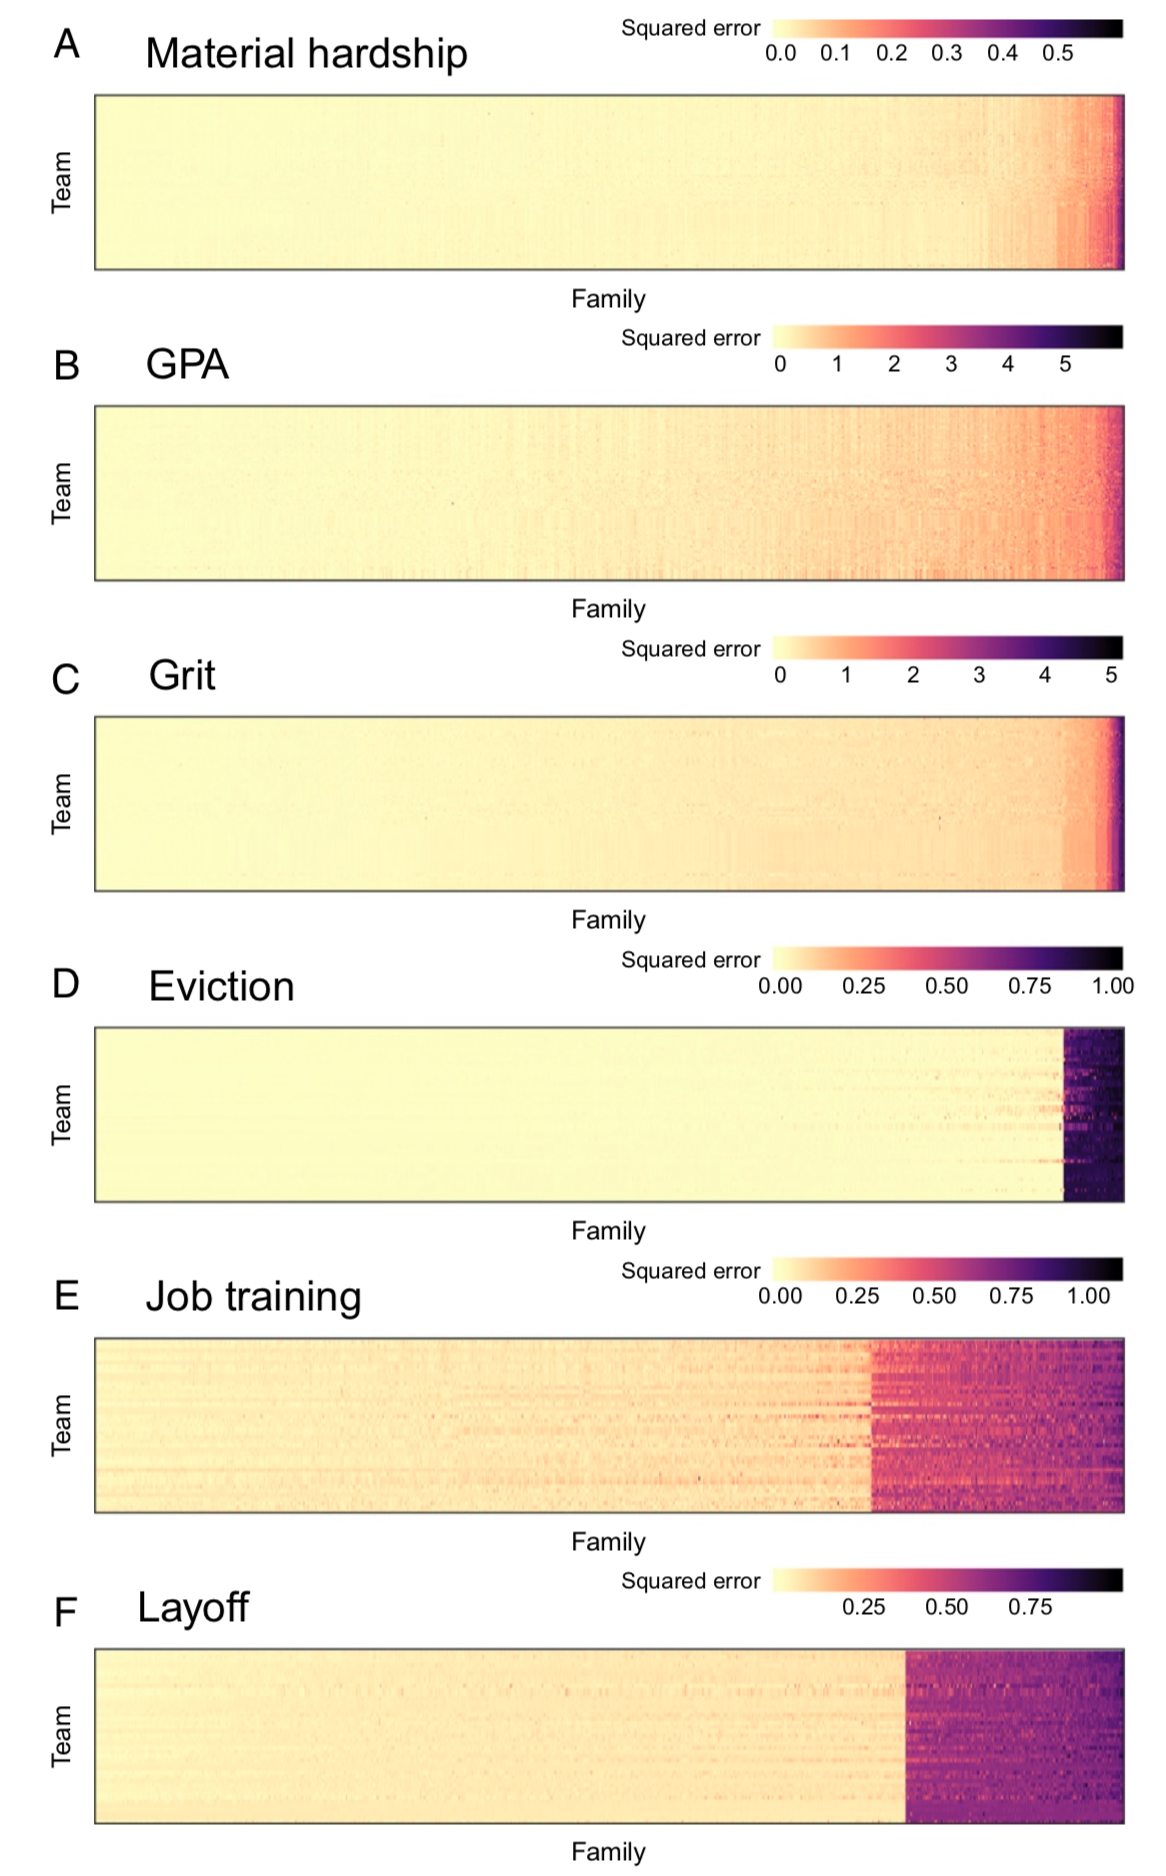
\includegraphics[height=0.9\textheight]{figures/salganik_measuring_2020_fig4}
\end{center}

\end{frame}
%%%%%%%%%%%%%%%%%%%%%%%%%%
\begin{frame}

\begin{center}
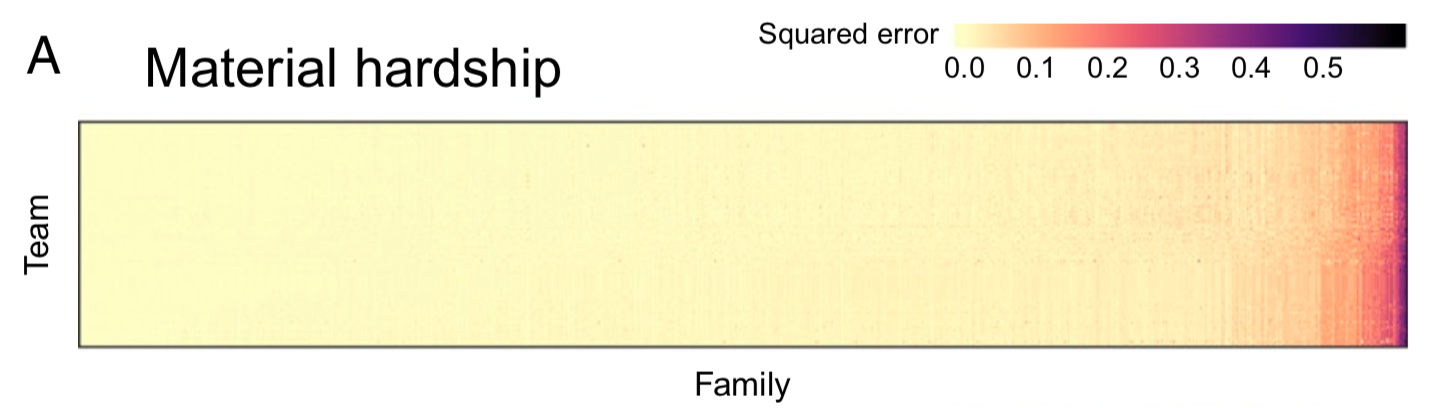
\includegraphics[width=\textwidth]{figures/salganik_measuring_2020_fig4a}
\end{center}

\vfill
Ensembling didn't improve things much. :(

\end{frame}
%%%%%%%%%%%%%%%%%%%%%%%%%%%%
\begin{frame}

\begin{center}
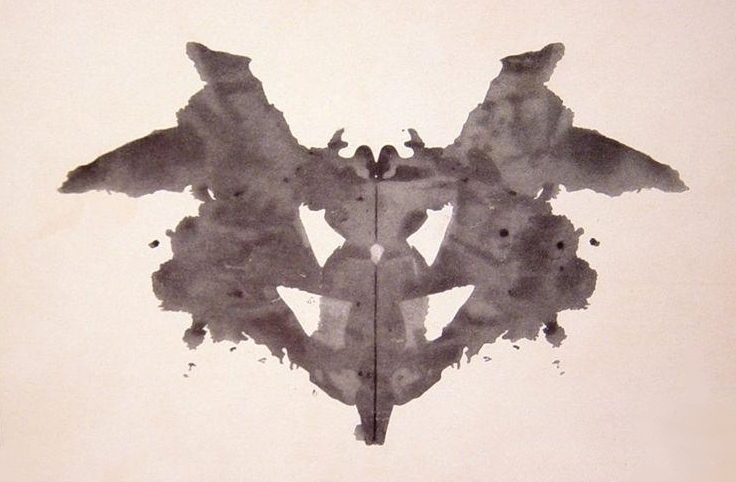
\includegraphics[height=\textheight]{figures/Rorschach_blot_01.jpg}
\end{center}

\vfill
\tiny{\url{https://commons.wikimedia.org/wiki/File:Rorschach_blot_01.jpg}}

\end{frame}
%%%%%%%%%%%%%%%%%%%%%%%%%%
\begin{frame}

Researchers must reconcile an ``understanding/prediction'' paradox \pause
\begin{itemize}
\item We don't understand much \pause
\item Prediction is not a good measure of understanding \pause
\item Our current understanding is correct but incomplete
\end{itemize}

\end{frame}
%%%%%%%%%%%%%%%%%%%%%%%%%%
\begin{frame}

Was the Fragile Families Challenge a success or failure?

\end{frame}
%%%%%%%%%%%%%%%%%%%%%%%%%%
\begin{frame}

Behind the scenes: Designing and running a mass collaboration

\end{frame}
%%%%%%%%%%%%%%%%%%%%%%%%%%%
\begin{frame}

Too hard, don't do it

\end{frame}
%%%%%%%%%%%%%%%%%%%%%%%%%%
\begin{frame}

Use a mix of approaches to get folks to participate

\begin{center}
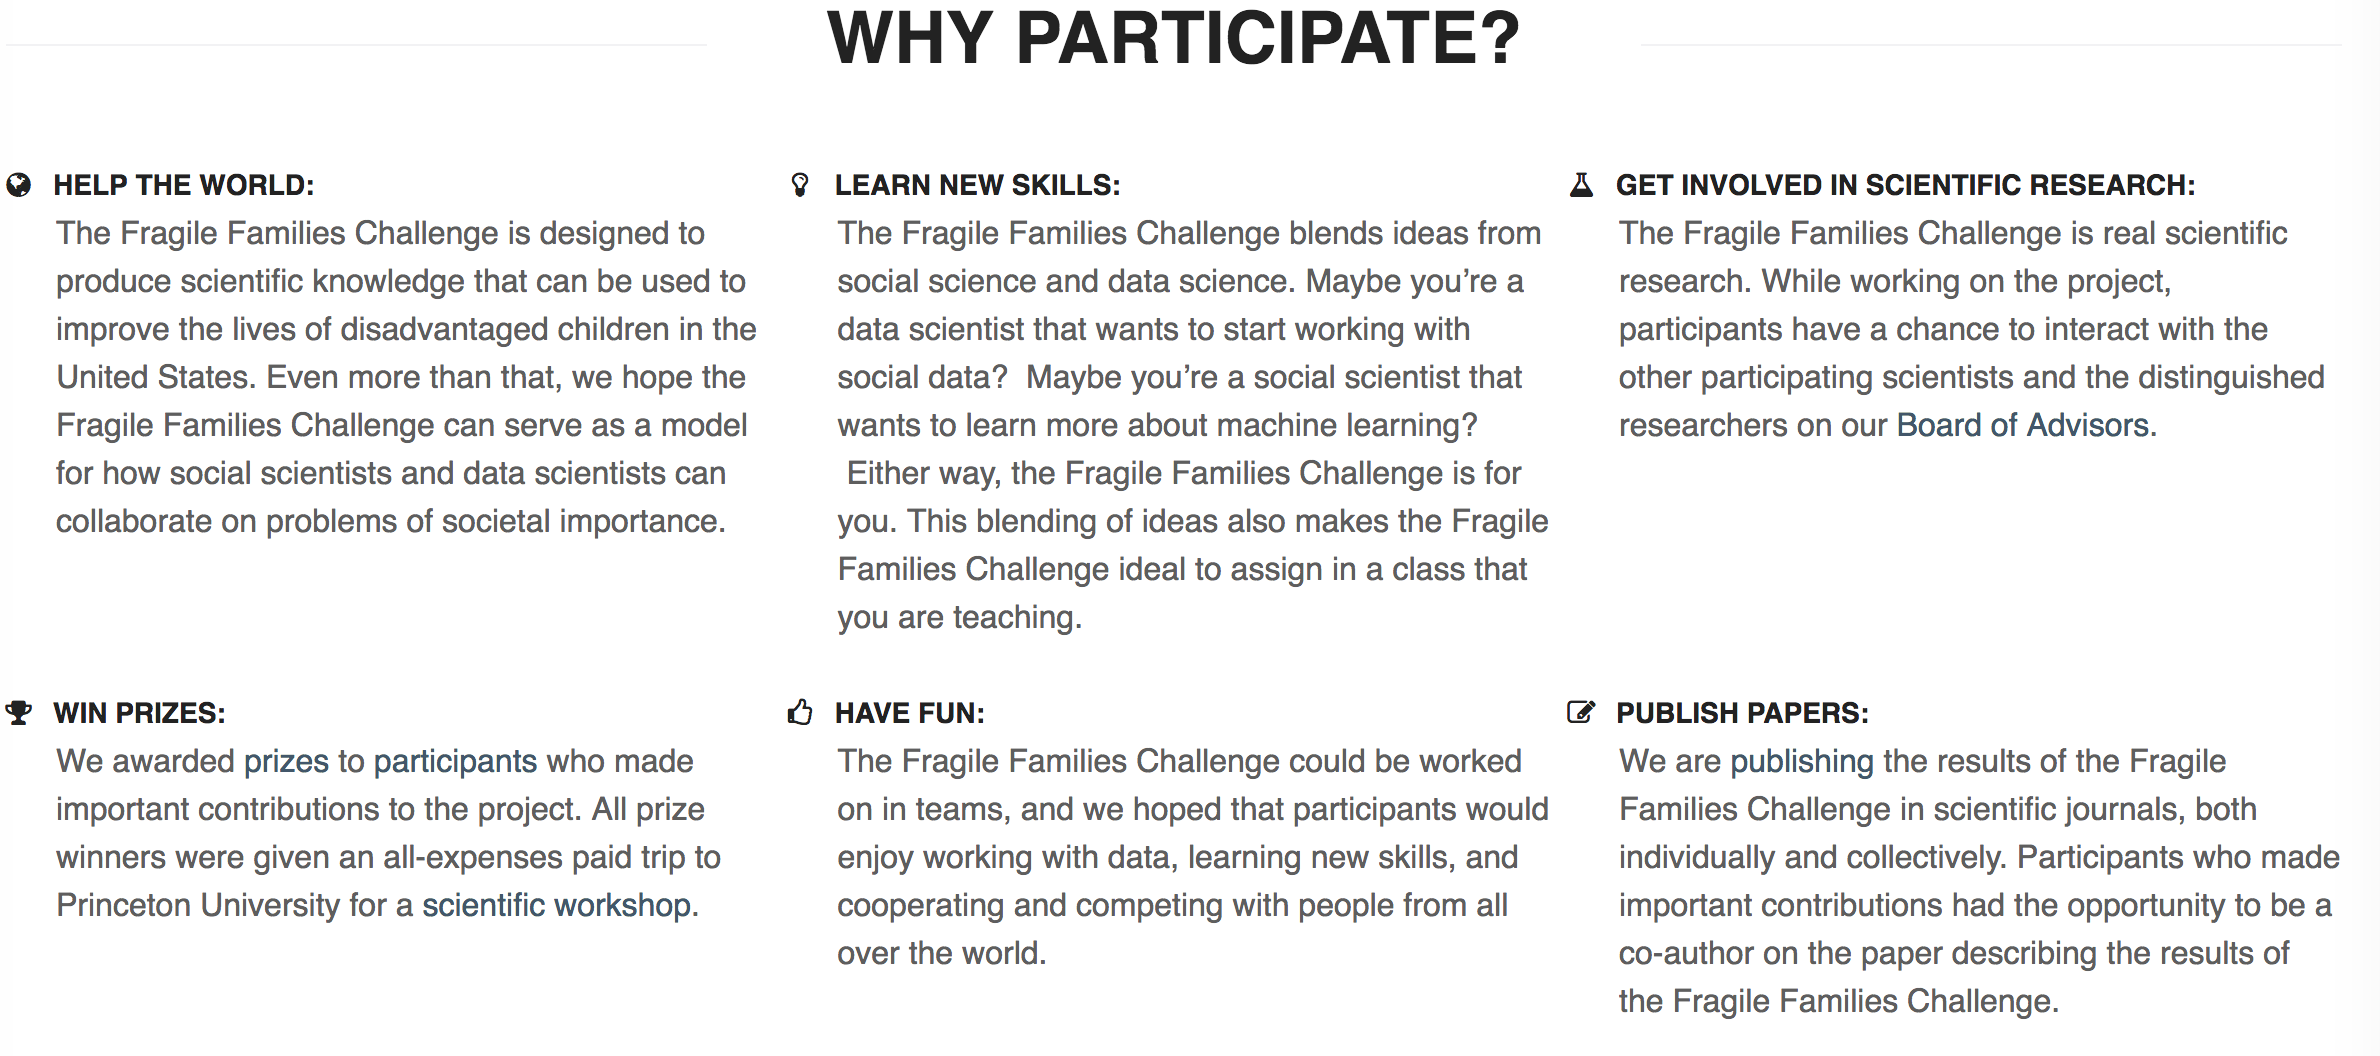
\includegraphics[width=\textwidth]{figures/ffc_why_participate}
\end{center}

\end{frame}
%%%%%%%%%%%%%%%%%%%%%%%%%%
\begin{frame}

``Hack'' existing scientific reward mechanisms: papers and prizes.\\

\begin{center}
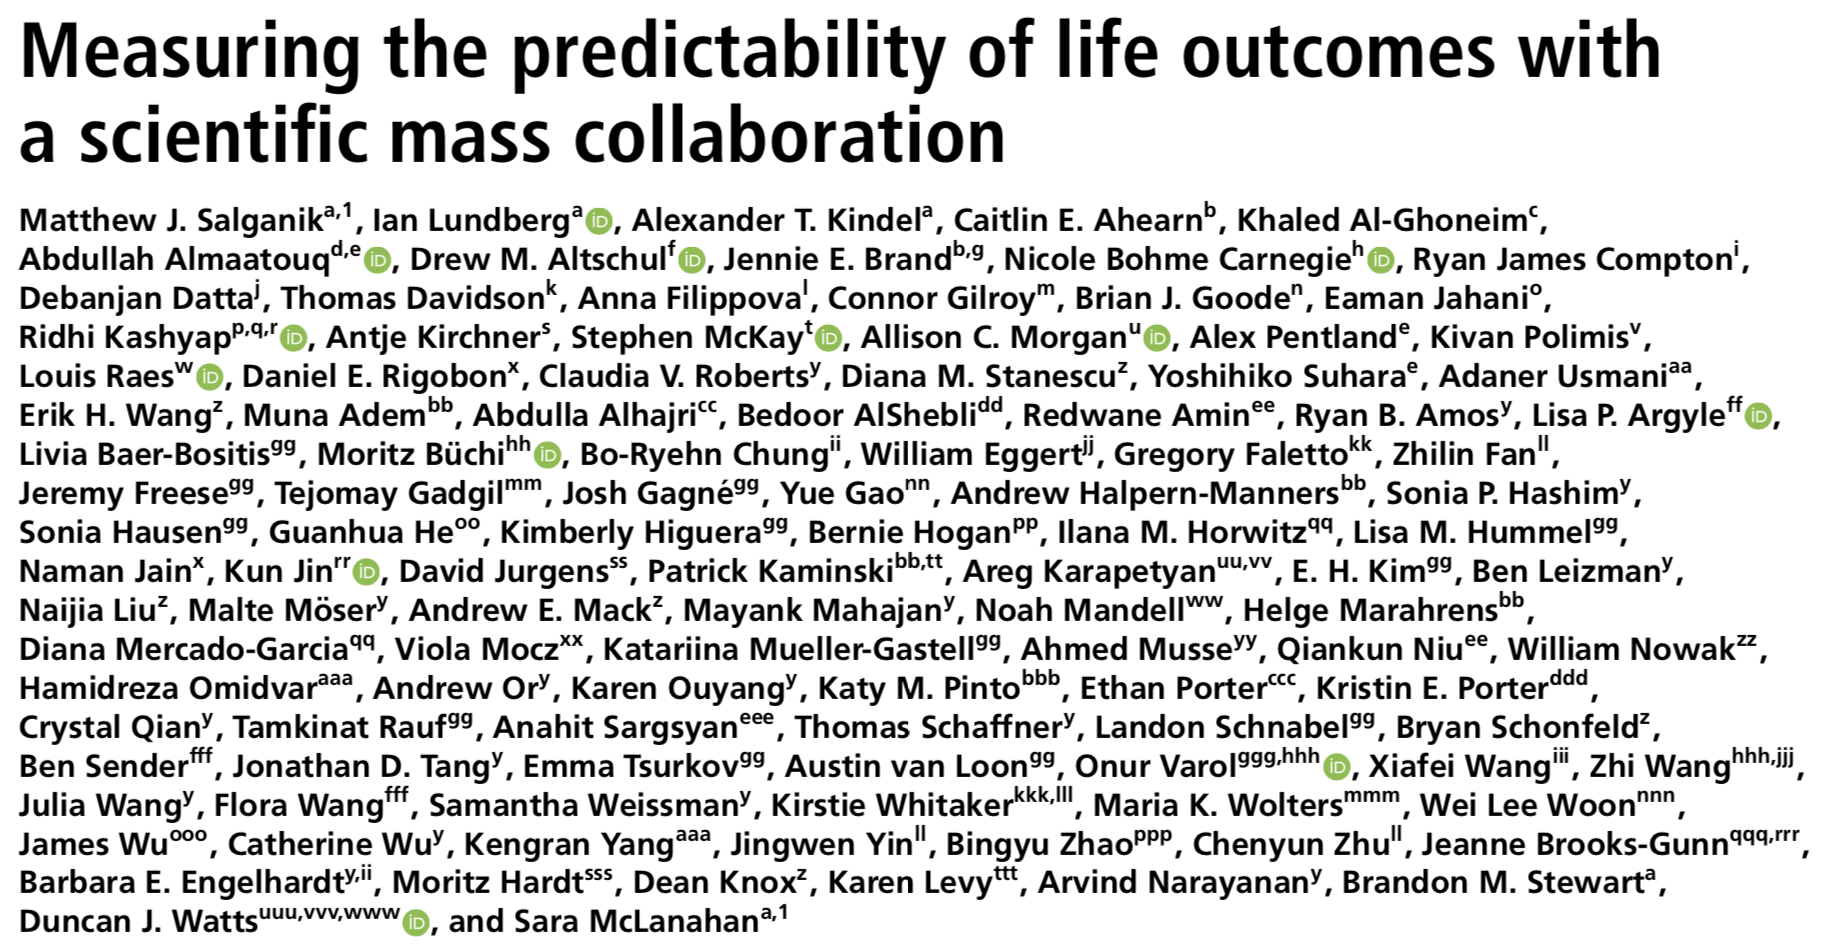
\includegraphics[width=0.3\textwidth]{figures/salganik_measuring_2020_title_authors}
\end{center}

\pause

\begin{center}

\includegraphics[width=0.3\textwidth]{figures/salganik_introduction_2019_title}
\end{center}

\pause

\begin{center}
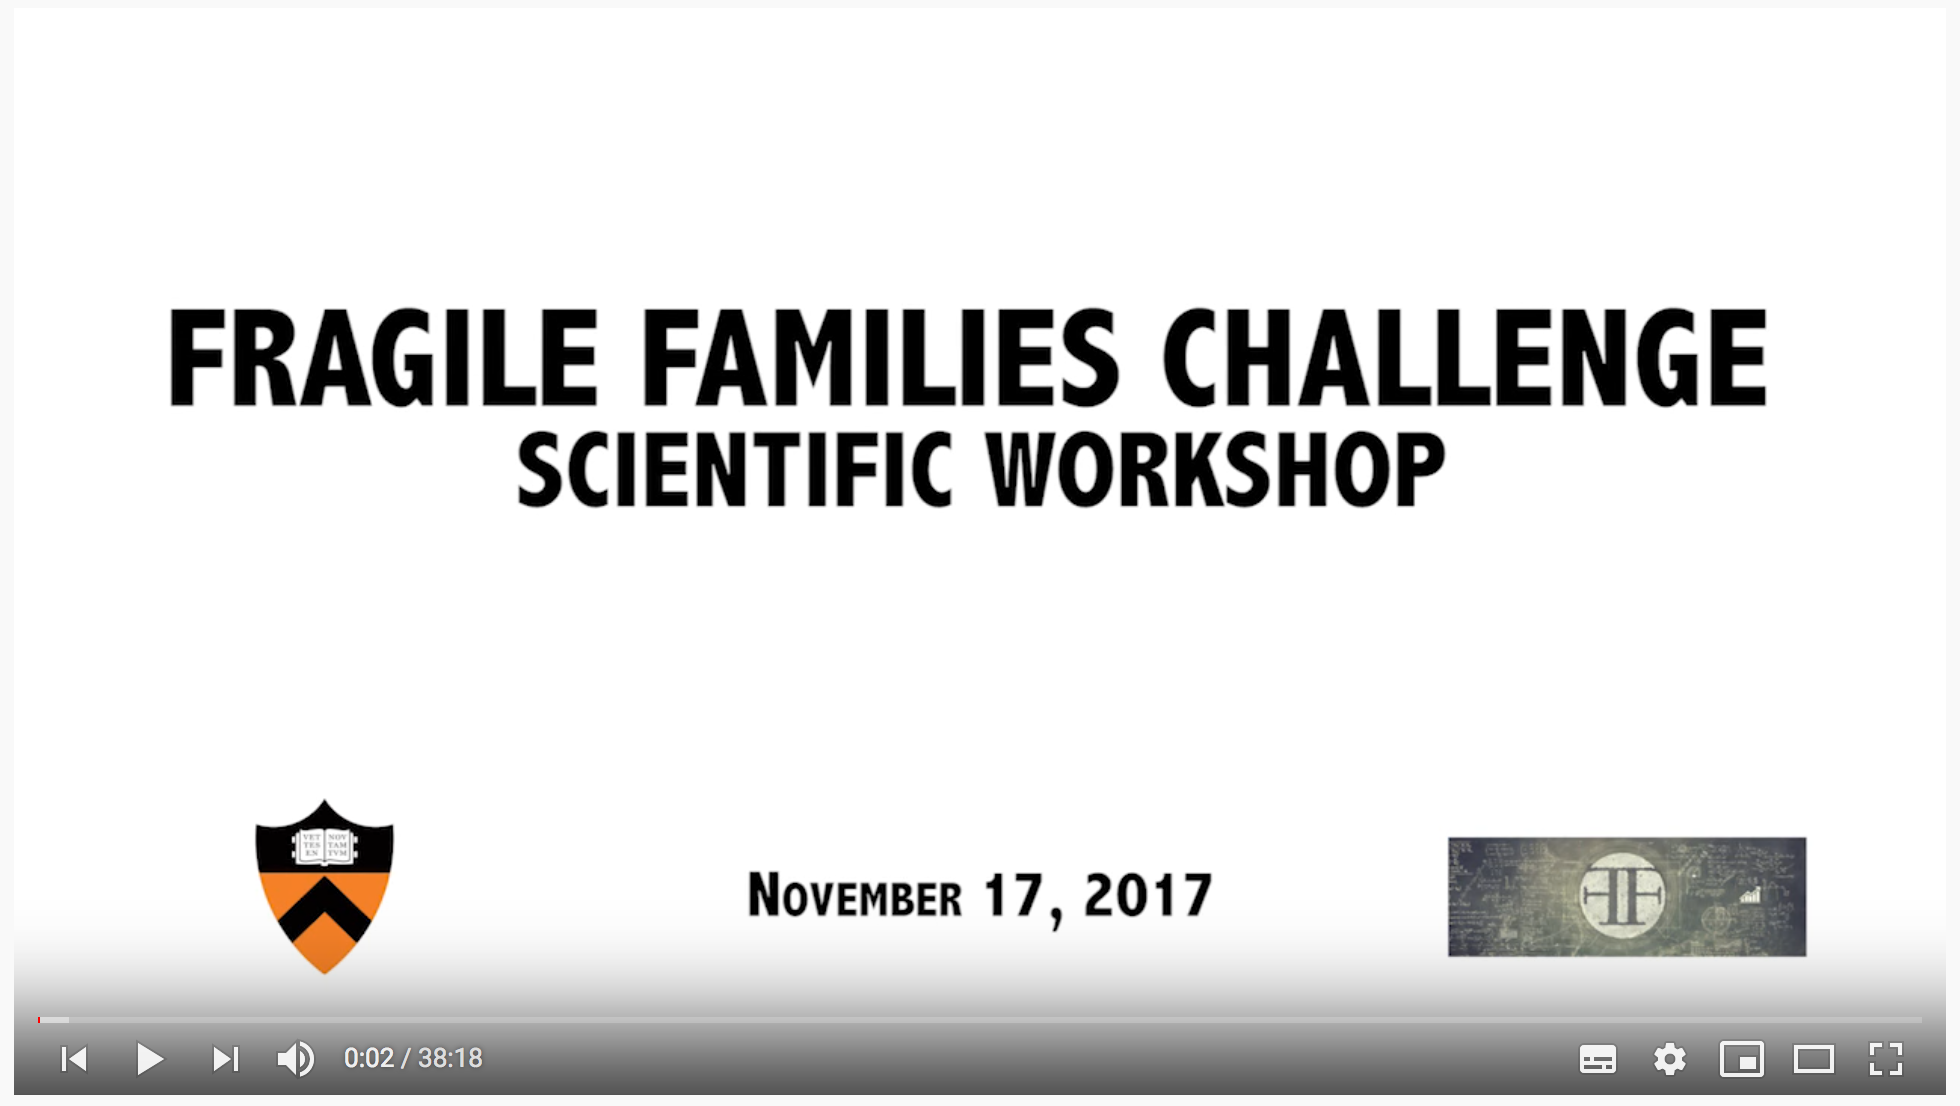
\includegraphics[width=0.3\textwidth]{figures/ffc_scientific_workshop}
\end{center}

\end{frame}
%%%%%%%%%%%%%%%%%%%%%%%
\begin{frame}

\begin{center}

\includegraphics[width=0.5\textwidth]{figures/lundberg_privacy_2019_title}
\end{center}

\pause
\vfill

\begin{center}
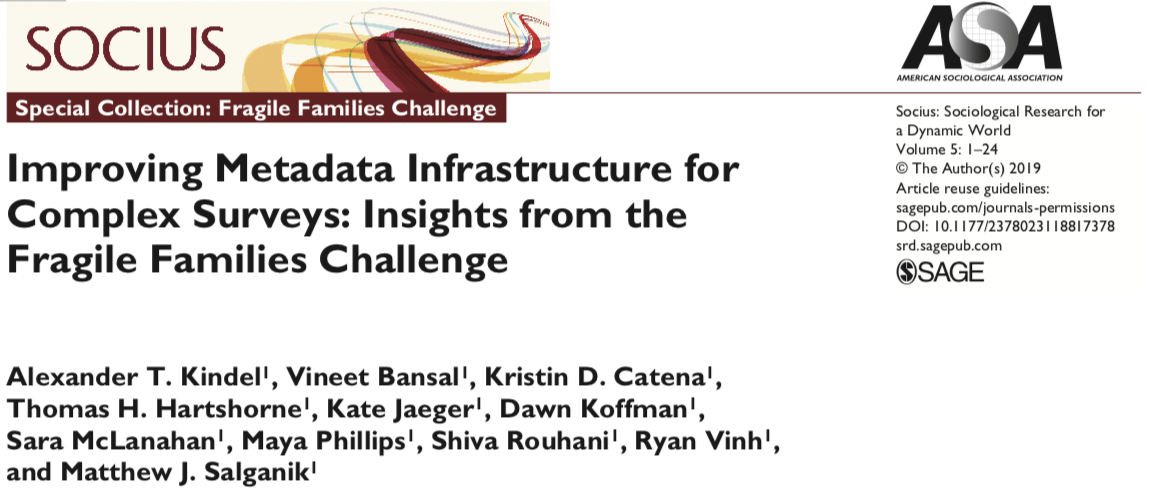
\includegraphics[width=0.5\textwidth]{figures/kindel_improving_2019_title}
\end{center}

\pause
\vfill

\begin{center}

\includegraphics[width=0.5\textwidth]{figures/liu_successes_2019_title}
\end{center}

\end{frame}
%%%%%%%%%%%%%%%%%%%%%%%
\begin{frame}

Competition vs collaboration
\begin{itemize}
\item We can learn from looking at the full set of submissions not just the best
\pause
\item We can open source everything to seed future research
\pause
\item Just feels right to me
\end{itemize}

\end{frame}
%%%%%%%%%%%%%%%%%%%%%%%%%%
\begin{frame}

Break into discussion groups

\end{frame}
%%%%%%%%%%%%%%%%%%%%%%%%%%
\begin{frame}

Getting ready for Thursday

\end{frame}
%%%%%%%%%%%%%%%%%%%%%%%%%%
\begin{frame}

Thoughts about reading the interviews
\begin{itemize}
\item Starts simple, gets more personal.  This is what happens when you talk to people. \pause
\item Year 15 interview GPA refers to 9th grade for both young adults.\pause
\item Difficulty of calibration. \pause
\item What is the goal of the reading? Filling out the sheet and helping us make sense of the results from the Challenge \pause
\item If you don't have access yet, let me know \pause
\item We will have guess on Thursday from the FFCWS data team and the dark matter interview team \pause
\end{itemize}

\end{frame}
%%%%%%%%%%%%%%%%%%%%%%%%%%




\frame{\titlepage}


\end{document}
